\subsubsection*{\underline{\textsc{\Large Ogre Zombie}}}
\noindent\emph{Large undead, neutral evil}

\noindent\rule{0.5\textwidth}{0.5pt}

\noindent\textbf{Armor Class}: 8

\noindent\textbf{Hit Points}: 85 (9d10 + 36)

\noindent\textbf{Speed}: 30 ft.

\noindent\rule{0.5\textwidth}{0.5pt} \\
\begin{table}[H]
	\begin{tabular}{cccccc}
		\textbf{STR} & \textbf{DEX} & \textbf{CON} & \textbf{INT} & \textbf{WIS} & \textbf{CHA} \\
		19 (+4) & 6 (-2) & 18 (+4) & 3 (-4) & 6 (-2) & 5 (-3) \\
	\end{tabular}
\end{table}
\noindent\rule{0.5\textwidth}{0.5pt} \\

\noindent\textbf{Saving Throws}: Wis +0

\noindent\textbf{Damage Immunities}: poison

\noindent\textbf{Condition Immunities}: poisoned

\noindent\textbf{Senses}: darkvision 60 ft., passive Perception 8

\noindent\textbf{Languages}: understands Common and Giant but can't speak

\noindent\textbf{Challenge}: 2 (450 XP)

\noindent\rule{0.5\textwidth}{0.5pt}

\noindent\textbf{Undead Fortitude}: If damage reduces the zombie to 0 hit points, it must make a Constitution saving throw with a DC of 5 + the damage taken, unless the damage is radiant or from a critical hit. On a success, the zombie drops to 1 hit point instead.

\noindent\rule{0.5\textwidth}{0.5pt}

\noindent\textbf{ACTIONS}

\noindent\textbf{Morningstar}: Melee Weapon Attack: +6 to hit, reach 5 ft., one target. Hit: 13 (2d8 + 4) bludgeoning damage.

\begin{center}
	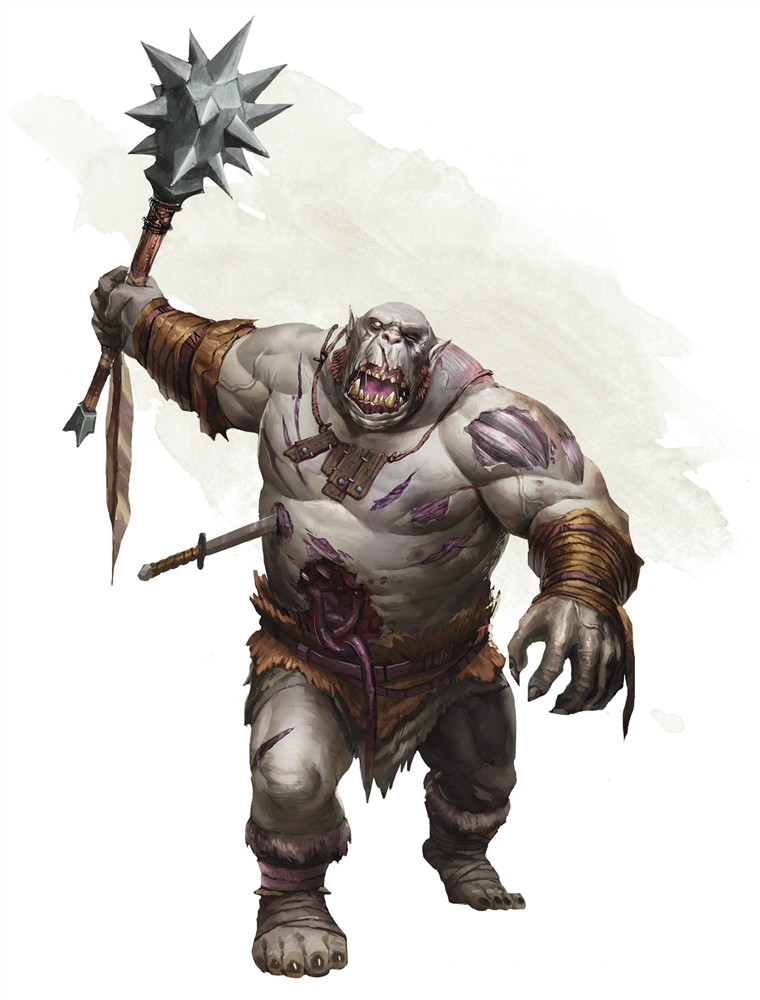
\includegraphics[width = 0.3\textwidth]{ogre-zombie}
	
	\emph{Ogre Zombie}
\end{center}